% ============================================================
% HÌNH VẼ CHƯƠNG 3 (TikZ) — gọi bằng macro trong Chap3.tex
%   \HinhUseCase     : biểu đồ ca sử dụng tổng quát        (fig:usecase)
%   \HinhOnOffChain  : phân tách dữ liệu on/off-chain       (fig:onoffchain)
%   \HinhTrangThai   : biểu đồ trạng thái của lô tín chỉ    (fig:trangthai)
% Đây là bản đề xuất theo phiếu giao nhiệm vụ: sửa lại cho khớp thiết kế thực tế của bạn.
% ============================================================

% Hình người (tác nhân UML)
\tikzset{
  tacnhan/.pic={
    \draw[thick] (0,0.62) circle (0.15);
    \draw[thick] (0,0.47) -- (0,0.05);
    \draw[thick] (-0.25,0.33) -- (0.25,0.33);
    \draw[thick] (0,0.05) -- (-0.18,-0.28);
    \draw[thick] (0,0.05) -- (0.18,-0.28);
  }
}

% ---------- Biểu đồ ca sử dụng tổng quát ----------
\newcommand{\HinhUseCase}{%
\begin{figure}[htbp]
\centering
\begin{tikzpicture}[font=\footnotesize]
  % Khung hệ thống
  \draw[thick] (3.0,-4.3) rectangle (9.8,4.6);
  \node[font=\footnotesize\bfseries] at (6.4,4.25) {Hệ thống quản lý tín chỉ các-bon};
  % Ca sử dụng: tên nút / tung độ / nội dung
  \foreach \ten/\y/\noidung in {
      uc1/3.5/{Thẩm định, phê duyệt và mint tín chỉ},
      uc2/2.6/{Đăng ký dự án},
      uc3/1.7/{Gửi yêu cầu cấp tín chỉ},
      uc4/0.8/{Nạp tín chỉ vào pool, đổi token},
      uc5/-0.1/{Mua bán, chuyển nhượng tín chỉ},
      uc6/-1.0/{Hủy tín chỉ để bù trừ (retire)},
      uc7/-1.9/{Tra cứu tín chỉ, chứng nhận hủy},
      uc8/-2.8/{Theo dõi dashboard hạn ngạch},
      uc9/-3.7/{Quản lý tài khoản, phân quyền}} {
    \draw (6.4,\y) ellipse (3.2cm and 0.38cm);
    \node at (6.4,\y) {\noidung};
    \coordinate (\ten-w) at (3.2,\y);
    \coordinate (\ten-e) at (9.6,\y);
  }
  % Tác nhân bên trái (tên ở dưới)
  \pic at (1.2,3.1) {tacnhan};   \node[align=center] at (1.2,2.55) {VVB};
  \pic at (1.2,0.8) {tacnhan};   \node[align=center] at (1.2,0.25) {Chủ dự án};
  % Tác nhân bên phải (tên ở bên phải để không đè lên đường nối)
  \pic at (11.2,0.5) {tacnhan};  \node[align=left, anchor=west] at (11.5,0.55) {Doanh nghiệp\\mua};
  \pic at (11.2,-3.0) {tacnhan}; \node[align=left, anchor=west] at (11.5,-2.95) {Cơ quan\\quản lý};
  % Liên kết
  \draw (1.5,3.4) -- (uc1-w);
  \foreach \u in {uc2,uc3,uc4,uc5} \draw (1.5,1.1) -- (\u-w);
  \foreach \u in {uc4,uc5,uc6,uc7} \draw (10.9,0.8) -- (\u-e);
  \foreach \u in {uc7,uc8,uc9} \draw (10.9,-2.7) -- (\u-e);
\end{tikzpicture}
\caption{Biểu đồ ca sử dụng tổng quát của hệ thống}
\label{fig:usecase}
\end{figure}}

% ---------- Phân tách dữ liệu on-chain / off-chain ----------
\newcommand{\HinhOnOffChain}{%
\begin{figure}[htbp]
\centering
\begin{tikzpicture}[
    >=Stealth,
    o/.style={draw, rounded corners=2pt, align=left, font=\footnotesize,
              text width=4.7cm, inner sep=4pt, fill=white},
    nhan/.style={font=\scriptsize, align=center, text width=2.6cm}]
  % Off-chain
  \node[o] (files) at (2.6,1.6) {\textbf{Kho tệp}\\
      IPFS hoặc lưu trữ đối tượng:\\
      PDD, báo cáo thẩm định,\\ tệp metadata JSON};
  \node[o, below=5mm of files] (db) {\textbf{CSDL quan hệ}\\
      PostgreSQL, theo mô hình\\ CAD Trust V2.0:\\
      Project, Stakeholders,\\ Verifications, Issuances, Units;\\
      tài khoản ứng dụng (bảng riêng);\\
      lịch sử giao dịch đồng bộ từ sự kiện};
  \node[draw, thick, dashed, rounded corners=4pt, inner sep=6pt, fit=(files)(db),
        label={[font=\footnotesize\bfseries]above:Off-chain (backend)}] (off) {};
  % On-chain
  \node[o, fill=gray!10] (nft) at (11.0,1.6) {\textbf{Hợp đồng NFT tín chỉ (ERC-721)}\\
      tokenId, chủ sở hữu, số sê-ri,\\ mã băm hồ sơ, URI metadata};
  \node[o, fill=gray!10, below=4mm of nft] (pool) {\textbf{Hợp đồng pool (ERC-20)}\\
      số dư token,\\ NFT đang khóa trong pool};
  \node[o, fill=gray!10, below=4mm of pool] (ret) {\textbf{Module Retirement}\\
      sự kiện Retired, người thụ hưởng};
  \node[draw, thick, rounded corners=4pt, inner sep=6pt, fit=(nft)(pool)(ret),
        label={[font=\footnotesize\bfseries]above:On-chain (Ethereum Sepolia)}] (on) {};
  % Luồng dữ liệu
  \draw[->, thick] (files.east) -- node[nhan, above] {mã băm hồ sơ (keccak256) và URI khi mint}
      (on.west |- files.east);
  \draw[->, thick] (on.west |- db.east) -- node[nhan, below] {sự kiện Minted, Transfer, Retired: backend đồng bộ}
      (db.east);
\end{tikzpicture}
\caption{Phân tách dữ liệu giữa phần on-chain và off-chain của hệ thống}
\label{fig:onoffchain}
\end{figure}}

% ---------- Biểu đồ trạng thái của một lô tín chỉ ----------
\newcommand{\HinhTrangThai}{%
\begin{figure}[htbp]
\centering
\begin{tikzpicture}[
    >=Stealth,
    tt/.style={draw, rounded corners=6pt, align=center, font=\footnotesize,
               minimum height=0.9cm, inner xsep=5pt, fill=white},
    nhan/.style={font=\scriptsize, align=center}]
  \node[circle, fill=black, inner sep=3pt] (bd) at (0,0) {};
  \node[tt] (nhap)   at (1.4,0)   {Nháp};
  \node[tt] (cho)    at (4.5,0)   {Chờ thẩm định};
  \node[tt] (tuchoi) at (4.5,-2.3) {Bị từ chối};
  \node[tt] (dacap)  at (9.0,0)   {Đã cấp\\(NFT ERC-721)};
  \node[tt] (pool)   at (9.0,-2.6) {Trong pool\\(ERC-20)};
  \node[tt] (dahuy)  at (12.6,0)   {Đã hủy\\(retired)};
  \node[circle, draw, inner sep=4pt] (kt) at (14.1,0) {};
  \node[circle, fill=black, inner sep=2pt] at (kt) {};

  \draw[->] (bd) -- (nhap);
  \draw[->] (nhap) -- node[nhan, above] {gửi\\hồ sơ} (cho);
  \draw[->] (cho) -- node[nhan, above] {VVB duyệt,\\mint NFT} (dacap);
  \draw[->] (cho) -- node[nhan, right] {VVB từ chối} (tuchoi);
  \draw[->] (tuchoi.west) -| node[nhan, pos=0.3, below] {bổ sung hồ sơ} (nhap.south);
  \draw[->] (dacap) -- node[nhan, above] {hủy hết\\(burn NFT)} (dahuy);
  \draw[->] (dahuy) -- (kt);
  \draw[->] ([xshift=-5mm]dacap.south) -- node[nhan, left] {nạp vào pool} ([xshift=-5mm]pool.north);
  \draw[->] ([xshift=5mm]pool.north) -- node[nhan, right] {đổi lại\\(redeem)} ([xshift=5mm]dacap.south);
  \draw[->] (pool.east) -| node[nhan, pos=0.3, below] {hủy hết phần còn lại\\ từ pool} (dahuy.south);
  \draw[->] ([xshift=-4mm]dacap.north) .. controls +(-0.3,0.9) and +(0.3,0.9) ..
      node[nhan, above] {chuyển nhượng; hủy một phần} ([xshift=4mm]dacap.north);
  \draw[->] ([xshift=-4mm]pool.south) .. controls +(-0.3,-0.9) and +(0.3,-0.9) ..
      node[nhan, below] {giao dịch token PCC; hủy một phần} ([xshift=4mm]pool.south);
\end{tikzpicture}
\caption{Biểu đồ trạng thái của một lô tín chỉ các-bon trong hệ thống}
\label{fig:trangthai}
\end{figure}}

% ============================================================
% HÌNH BỔ SUNG GIAI ĐOẠN 3–4 (vẽ theo mã nguồn thực tế trong contracts/ và backend/)
%   \HinhLopHopDong   : biểu đồ lớp các hợp đồng thông minh   (fig:lophopdong)
%   \HinhERD          : lược đồ CSDL off-chain                 (fig:erd)
%   \HinhTuanTuMint   : tuần tự yêu cầu cấp – thẩm định – mint (fig:tuantu-mint)
%   \HinhTuanTuRetire : tuần tự nạp pool – giao dịch – hủy     (fig:tuantu-retire)
%   \BangAPI          : bảng endpoint API REST                 (tab:api)
% ============================================================

% Hộp lớp UML: tên / thuộc tính / phương thức
\newcommand{\lopUML}[3]{%
  \begin{tabular}{@{}l@{}}
    \multicolumn{1}{c}{\textbf{#1}}\\ \hline
    \rule{0pt}{2.4ex}#2\\ \hline
    \rule{0pt}{2.4ex}#3
  \end{tabular}}

\newcommand{\HinhLopHopDong}{%
\begin{figure}[htbp]
\centering
\begin{adjustbox}{max width=\textwidth}
\begin{tikzpicture}[
    >=Stealth, font=\scriptsize,
    lop/.style={draw, fill=white, inner sep=3pt, align=left},
    oz/.style={draw, dashed, rounded corners=2pt, inner sep=3pt, font=\scriptsize\itshape, fill=gray!8},
    ke/.style={-{Triangle[open]}, thick},
    dung/.style={->, dashed}]
  % Thư viện OpenZeppelin
  \node[oz] (erc721) at (0.2,4.8) {ERC721URIStorage};
  \node[oz] (ac)     at (3.0,4.8) {AccessControl};
  \node[oz] (pa)     at (5.4,4.8) {Pausable};
  \node[oz] (erc20)  at (9.8,4.8) {ERC20};
  \node[oz] (recv)   at (12.2,4.8) {IERC721Receiver};
  \node[oz] (rg)     at (15.0,4.8) {ReentrancyGuard};

  \node[lop, anchor=north] (nft) at (2.8,3.8) {\lopUML{CarbonCreditNFT}{%
      + VERIFIER\_ROLE, RETIREMENT\_AGENT\_ROLE : bytes32\\
      - \_batches : mapping(uint256 $\Rightarrow$ CreditBatch)\\
      - \_certificates : RetirementCertificate[]\\
      + nextAvailableSerial : mapping(bytes32 $\Rightarrow$ uint256)\\
      + documentUsed : mapping(bytes32 $\Rightarrow$ bool)}{%
      + mintBatch(to, projectId, vintage, serialFrom, quantity,\\
      \quad documentHash, uri) : uint256 \quad \textit{onlyRole(VERIFIER)}\\
      + retire(tokenId, amount, beneficiary, reason) : uint256\\
      + retireFor(retiree, tokenId, amount, beneficiary, reason)\\
      \quad \textit{onlyRole(RETIREMENT\_AGENT)}\\
      + pause(), unpause() \quad \textit{onlyRole(DEFAULT\_ADMIN)}\\
      + getBatch(tokenId), remainingOf(tokenId), getCertificate(id)\\
      \textit{sự kiện:} CreditMinted, CreditRetired}};

  \node[lop, anchor=north] (pool) at (12.4,3.8) {\lopUML{CarbonPool}{%
      + credits : CarbonCreditNFT \quad \textit{immutable}\\
      - \_pooled : EnumerableSet.UintSet\\
      + decimals() = 0 \quad (1 PCC = 1 tCO$_2$e)}{%
      + deposit(tokenId)\\
      + onERC721Received(...) : đúc PCC cho người nạp\\
      + redeem(tokenId) : đốt PCC, trả NFT\\
      + retire(tokenId, amount, beneficiary, reason)\\
      + pooledTokenIds(), isPooled(tokenId)\\
      \textit{sự kiện:} Deposited, Redeemed, RetiredFromPool}};

  \node[lop, anchor=north] (batch) at (2.8,-2.6) {\lopUML{$\ll$struct$\gg$ CreditBatch}{%
      projectId : string; vintage : uint16\\
      serialFrom, quantity, retired : uint256\\
      documentHash : bytes32; verifier : address\\
      issuedAt : uint64}{\textit{(dữ liệu của một lô)}}};

  \node[lop, anchor=north] (cert) at (12.4,-1.4) {\lopUML{$\ll$struct$\gg$ RetirementCertificate}{%
      tokenId, serialFrom, serialTo, amount : uint256\\
      retiree : address\\
      beneficiary, reason : string; retiredAt : uint64}{\textit{(một chứng nhận hủy)}}};

  \draw[ke] ([xshift=-2.6cm]nft.north) -- (erc721.south);
  \draw[ke] ([xshift=0.2cm]nft.north) -- (ac.south);
  \draw[ke] ([xshift=2.6cm]nft.north) -- (pa.south);
  \draw[ke] ([xshift=-2.6cm]pool.north) -- (erc20.south);
  \draw[ke] ([xshift=-0.2cm]pool.north) -- (recv.south);
  \draw[ke] ([xshift=2.6cm]pool.north) -- (rg.south);
  \draw[dung] (pool.west) -- node[above, align=center] {gọi retireFor,\\ safeTransferFrom} (nft.east |- pool.west);
  \draw[-{Diamond[open]}] (batch.north) -- (nft.south);
  \draw[-{Diamond[open]}] (cert.west) -- ++(-1.2,0) |- ([yshift=4mm]nft.south east);
\end{tikzpicture}
\end{adjustbox}
\caption{Biểu đồ lớp của các hợp đồng thông minh}
\label{fig:lophopdong}
\end{figure}}

% ---------- Lược đồ CSDL ----------
% Bảng ERD: tên bảng / danh sách cột (khóa chính in đậm, khóa ngoại in nghiêng)
\newcommand{\bangERD}[2]{%
  \begin{tabular}{@{}l@{}}
    \multicolumn{1}{c}{\textbf{#1}}\\ \hline
    \rule{0pt}{2.2ex}#2
  \end{tabular}}

\newcommand{\HinhERD}{%
\begin{figure}[htbp]
\centering
\begin{adjustbox}{max width=\textwidth}
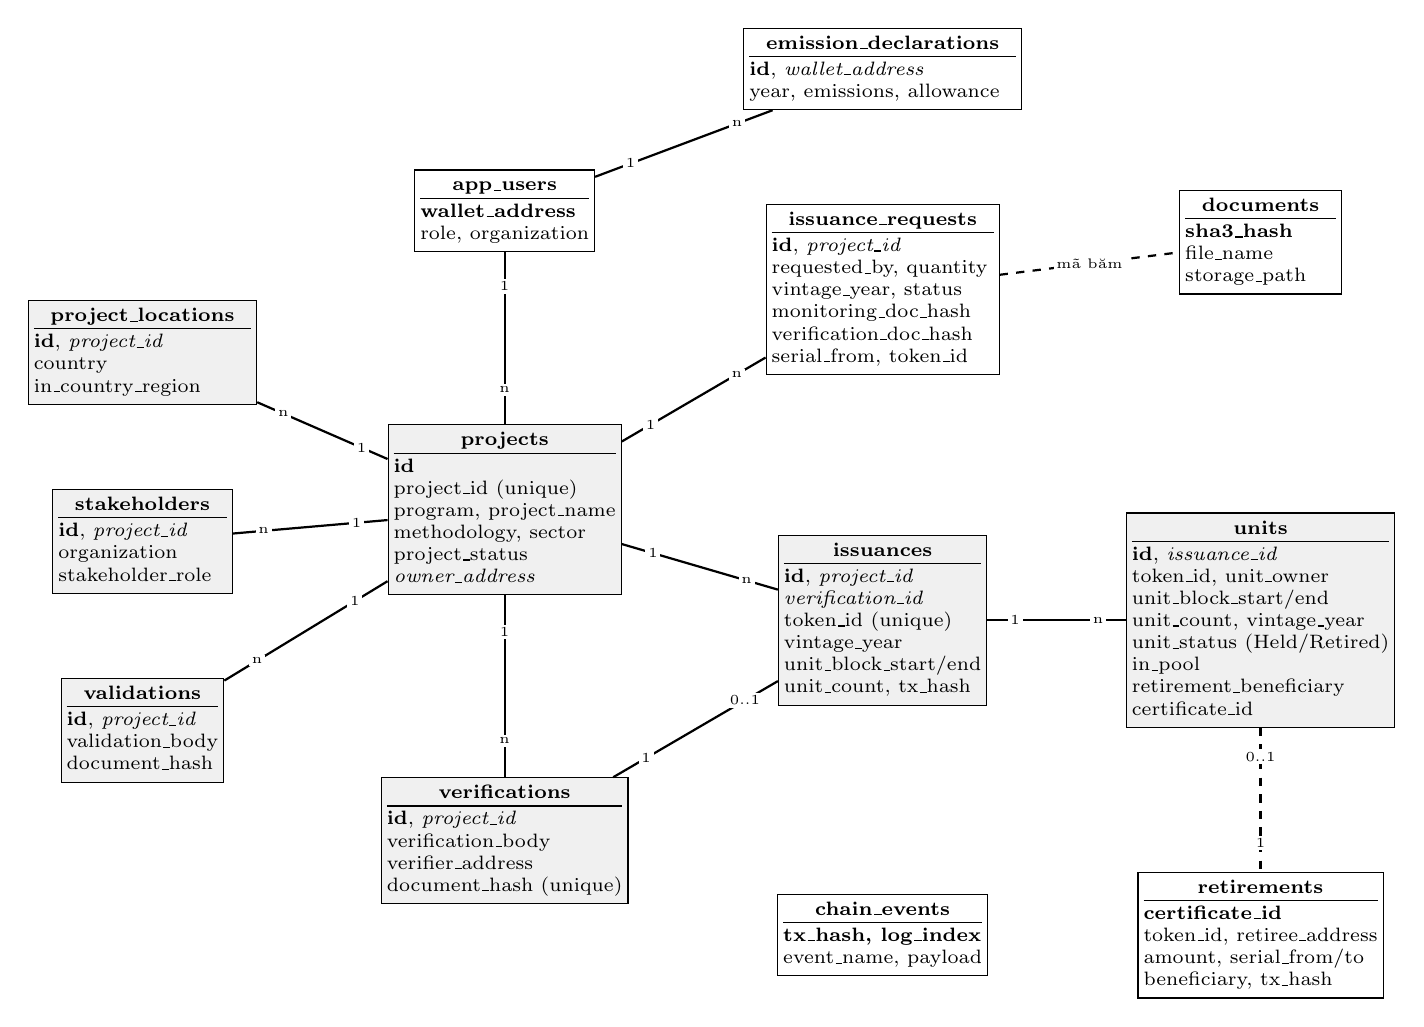
\begin{tikzpicture}[font=\scriptsize,
    bang/.style={draw, fill=white, inner sep=2pt, align=left},
    cad/.style={bang, fill=gray!12},
    lk/.style={draw, thick},
    n/.style={font=\tiny, fill=white, inner sep=1pt}]
  % Nhóm CAD Trust (nền xám)
  \node[cad] (proj) at (0,0) {\bangERD{projects}{%
     \textbf{id}\\ project\_id (unique)\\ program, project\_name\\ methodology, sector\\
     project\_status\\ \textit{owner\_address}}};
  \node[cad] (loc) at (-4.6,2.0) {\bangERD{project\_locations}{\textbf{id}, \textit{project\_id}\\ country\\ in\_country\_region}};
  \node[cad] (sh)  at (-4.6,-0.4) {\bangERD{stakeholders}{\textbf{id}, \textit{project\_id}\\ organization\\ stakeholder\_role}};
  \node[cad] (val) at (-4.6,-2.8) {\bangERD{validations}{\textbf{id}, \textit{project\_id}\\ validation\_body\\ document\_hash}};
  \node[cad] (ver) at (0,-4.2) {\bangERD{verifications}{\textbf{id}, \textit{project\_id}\\ verification\_body\\ verifier\_address\\ document\_hash (unique)}};
  \node[cad] (iss) at (4.8,-1.4) {\bangERD{issuances}{\textbf{id}, \textit{project\_id}\\ \textit{verification\_id}\\ token\_id (unique)\\ vintage\_year\\ unit\_block\_start/end\\ unit\_count, tx\_hash}};
  \node[cad] (unit) at (9.6,-1.4) {\bangERD{units}{\textbf{id}, \textit{issuance\_id}\\ token\_id, unit\_owner\\ unit\_block\_start/end\\ unit\_count, vintage\_year\\ unit\_status (Held/Retired)\\ in\_pool\\ retirement\_beneficiary\\ certificate\_id}};
  % Nhóm riêng của ứng dụng (nền trắng)
  \node[bang] (user) at (0,3.8) {\bangERD{app\_users}{\textbf{wallet\_address}\\ role, organization}};
  \node[bang] (req)  at (4.8,2.8) {\bangERD{issuance\_requests}{\textbf{id}, \textit{project\_id}\\ requested\_by, quantity\\ vintage\_year, status\\ monitoring\_doc\_hash\\ verification\_doc\_hash\\ serial\_from, token\_id}};
  \node[bang] (doc)  at (9.6,3.4) {\bangERD{documents}{\textbf{sha3\_hash}\\ file\_name\\ storage\_path}};
  \node[bang] (ret)  at (9.6,-5.4) {\bangERD{retirements}{\textbf{certificate\_id}\\ token\_id, retiree\_address\\ amount, serial\_from/to\\ beneficiary, tx\_hash}};
  \node[bang] (emi)  at (4.8,5.6) {\bangERD{emission\_declarations}{\textbf{id}, \textit{wallet\_address}\\ year, emissions, allowance}};
  \node[bang] (evt)  at (4.8,-5.4) {\bangERD{chain\_events}{\textbf{tx\_hash, log\_index}\\ event\_name, payload}};

  \draw[lk] (proj) -- node[n, pos=0.2]{1} node[n, pos=0.8]{n} (loc);
  \draw[lk] (proj) -- node[n, pos=0.2]{1} node[n, pos=0.8]{n} (sh);
  \draw[lk] (proj) -- node[n, pos=0.2]{1} node[n, pos=0.8]{n} (val);
  \draw[lk] (proj) -- node[n, pos=0.2]{1} node[n, pos=0.8]{n} (ver);
  \draw[lk] (proj) -- node[n, pos=0.2]{1} node[n, pos=0.8]{n} (iss);
  \draw[lk] (ver) -- node[n, pos=0.2]{1} node[n, pos=0.8]{0..1} (iss);
  \draw[lk] (iss) -- node[n, pos=0.2]{1} node[n, pos=0.8]{n} (unit);
  \draw[lk] (user) -- node[n, pos=0.2]{1} node[n, pos=0.8]{n} (proj);
  \draw[lk] (proj) -- node[n, pos=0.2]{1} node[n, pos=0.8]{n} (req);
  \draw[lk] (user) -- node[n, pos=0.2]{1} node[n, pos=0.8]{n} (emi);
  \draw[lk, dashed] (unit) -- node[n, pos=0.2]{0..1} node[n, pos=0.8]{1} (ret);
  \draw[lk, dashed] (req) -- node[n]{mã băm} (doc);
\end{tikzpicture}
\end{adjustbox}
\caption{Lược đồ cơ sở dữ liệu off-chain (nền xám: các bảng theo mô hình CAD Trust V2.0)}
\label{fig:erd}
\end{figure}}

% ---------- Biểu đồ tuần tự ----------
% \dongdoi{tên nút}{x}{nhãn}{y cuối}: vẽ một đường đời (lifeline)
\newcommand{\dongdoi}[4]{%
  \node[draw, fill=white, minimum width=1.9cm, minimum height=0.7cm, align=center, font=\scriptsize] (#1) at (#2,0) {#3};
  \draw[dashed, gray] (#1.south) -- (#2,#4);}
% \tinnhan[kiểu mũi tên]{x1}{x2}{y}{nhãn}
\newcommand{\tinnhan}[5][->]{%
  \draw[#1, >=Stealth] (#2,#4) -- node[above, font=\scriptsize, align=center] {#5} (#3,#4);}

\newcommand{\HinhTuanTuMint}{%
\begin{figure}[htbp]
\centering
\begin{adjustbox}{max width=\textwidth}
\begin{tikzpicture}[yscale=1.2]
  \dongdoi{cda}{0}{Chủ dự án\\(trình duyệt)}{-11.0}
  \dongdoi{be}{4.0}{Backend API}{-11.0}
  \dongdoi{db}{7.0}{PostgreSQL}{-11.0}
  \dongdoi{vvb}{10.0}{VVB\\(MetaMask)}{-11.0}
  \dongdoi{sc}{13.2}{CarbonCreditNFT}{-11.0}
  \dongdoi{ix}{16.4}{Bộ đồng bộ\\sự kiện}{-11.0}
  \tinnhan{0}{4.0}{-1.2}{POST /documents (báo cáo giám sát)}
  \tinnhan[<-]{0}{4.0}{-1.8}{sha3\_hash}
  \tinnhan{0}{4.0}{-2.5}{POST /issuance-requests}
  \tinnhan{4.0}{7.0}{-3.0}{INSERT, status = SUBMITTED}
  \tinnhan[<-]{4.0}{10.0}{-3.8}{GET /issuance-requests (danh sách chờ)}
  \tinnhan[<-]{4.0}{10.0}{-4.5}{POST /documents (báo cáo thẩm định)}
  \tinnhan[<-]{4.0}{10.0}{-5.2}{POST /issuance-requests/:id/approve}
  \tinnhan{4.0}{7.0}{-6.1}{kiểm tra mã băm chưa dùng;\\ INSERT verifications; APPROVED}
  \tinnhan{4.0}{10.0}{-7.0}{tham số mint (to, projectId, vintage,\\ serialFrom, quantity, documentHash, uri)}
  \tinnhan{10.0}{13.2}{-7.6}{mintBatch(...) ký bằng ví VVB}
  \node[draw, fill=white, font=\scriptsize, align=left, anchor=west] at (13.35,-8.3) {kiểm tra VERIFIER\_ROLE,\\ sê-ri không chồng lấn,\\ documentHash chưa dùng};
  \tinnhan{13.2}{16.4}{-9.4}{sự kiện CreditMinted, Transfer}
  \draw[->, >=Stealth] (16.4,-10.0) -- node[above, font=\scriptsize, align=center, pos=0.3] {INSERT issuances, units (Held); yêu cầu $\rightarrow$ MINTED} (7.0,-10.0);
  \tinnhan[<-]{0}{4.0}{-10.6}{trạng thái MINTED, lô \#tokenId}
\end{tikzpicture}
\end{adjustbox}
\caption{Biểu đồ tuần tự quy trình yêu cầu cấp, thẩm định và phát hành tín chỉ}
\label{fig:tuantu-mint}
\end{figure}}

\newcommand{\HinhTuanTuRetire}{%
\begin{figure}[htbp]
\centering
\begin{adjustbox}{max width=\textwidth}
\begin{tikzpicture}[yscale=1.2]
  \dongdoi{cda}{0}{Chủ dự án\\(MetaMask)}{-9.4}
  \dongdoi{dn}{3.4}{Doanh nghiệp\\(MetaMask)}{-9.4}
  \dongdoi{pool}{7.0}{CarbonPool\\(ERC-20)}{-9.4}
  \dongdoi{nft}{10.6}{CarbonCreditNFT\\(ERC-721)}{-9.4}
  \dongdoi{ix}{14.2}{Bộ đồng bộ\\+ CSDL}{-9.4}
  \tinnhan{0}{10.6}{-1.2}{safeTransferFrom(chủ dự án, pool, tokenId)}
  \tinnhan[<-]{7.0}{10.6}{-1.9}{onERC721Received(from, tokenId)}
  \node[draw, fill=white, font=\scriptsize, align=left, anchor=east] at (6.85,-2.6) {\_mint(from, remainingOf(tokenId));\\ NFT bị khóa trong pool};
  \tinnhan{0}{7.0}{-3.6}{transfer(doanh nghiệp, 300): bán từng phần}
  \tinnhan{3.4}{7.0}{-4.5}{retire(tokenId, 300, ...)}
  \node[draw, fill=white, font=\scriptsize, align=left, anchor=east] at (6.85,-5.1) {\_burn(doanh nghiệp, 300)};
  \tinnhan{7.0}{10.6}{-5.8}{retireFor(doanh nghiệp, tokenId, 300, ...)}
  \node[draw, fill=white, font=\scriptsize, align=left, anchor=west] at (10.75,-6.6) {retired += 300; lưu chứng nhận\\ (sê-ri, người hủy, thụ hưởng);\\ hủy hết thì \_burn(tokenId)};
  \tinnhan{10.6}{14.2}{-7.9}{sự kiện CreditRetired, Transfer}
  \tinnhan[<-]{3.4}{14.2}{-8.6}{GET /api/retirements/:id: chứng nhận hủy công khai}
\end{tikzpicture}
\end{adjustbox}
\caption{Biểu đồ tuần tự giao dịch qua pool và hủy tín chỉ}
\label{fig:tuantu-retire}
\end{figure}}

% ---------- Bảng API ----------
\newcommand{\BangAPI}{%
\begingroup\small
\renewcommand{\arraystretch}{1.15}
\begin{longtable}{|p{1.35cm}|>{\footnotesize}p{5.6cm}|>{\footnotesize\raggedright\arraybackslash}p{2.3cm}|>{\raggedright\arraybackslash}p{3.9cm}|}
\caption{Các endpoint của API REST}\label{tab:api}\\
\hline
\textbf{HTTP} & \textbf{Đường dẫn} & \textbf{Quyền} & \textbf{Chức năng}\\ \hline
\endfirsthead
\hline
\textbf{HTTP} & \textbf{Đường dẫn} & \textbf{Quyền} & \textbf{Chức năng}\\ \hline
\endhead
POST & /api/auth/nonce & Công khai & Lấy thông điệp đăng nhập cần ký\\ \hline
POST & /api/auth/login & Công khai & Xác minh chữ ký ví, cấp JWT; tạo tài khoản lần đầu\\ \hline
GET & /api/auth/me & Đã đăng nhập & Thông tin tài khoản\\ \hline
GET & /api/users & ADMIN & Danh sách tài khoản\\ \hline
PATCH & /api/users/:address/role & ADMIN & Đổi vai trò\\ \hline
GET & /api/projects & Công khai & Danh sách dự án kèm tổng đã cấp, đã hủy\\ \hline
GET & /api/projects/:id & Công khai & Chi tiết dự án, vị trí, các bên, thẩm định, đợt cấp\\ \hline
POST & /api/projects & PROJECT\_\allowbreak OWNER & Đăng ký dự án\\ \hline
PATCH & /api/projects/:id & Chủ dự án, ADMIN & Sửa thông tin; ADMIN đổi trạng thái\\ \hline
POST & /api/documents & Đã đăng nhập & Tải hồ sơ, trả mã băm keccak256\\ \hline
GET & /api/documents/:hash & Công khai & Thông tin, tải hồ sơ để đối chiếu mã băm\\ \hline
POST & /api/issuance-requests & PROJECT\_\allowbreak OWNER & Gửi yêu cầu cấp tín chỉ\\ \hline
GET & /api/issuance-requests[/:id] & Chủ dự án, VVB, ADMIN & Xem yêu cầu (kèm tham số mint nếu đã duyệt)\\ \hline
POST & /api/issuance-requests/:id/approve & VERIFIER & Phê duyệt, ghi thẩm định, trả tham số mint\\ \hline
POST & /api/issuance-requests/:id/reject & VERIFIER & Từ chối kèm lý do\\ \hline
GET & /api/issuances & Công khai & Danh sách đợt cấp\\ \hline
GET & /api/units & Công khai & Khối tín chỉ, lọc theo chủ sở hữu, trạng thái, lô, pool\\ \hline
GET & /api/units/lookup & Công khai & Tra cứu một số sê-ri\\ \hline
GET & /api/retirements[/:id] & Công khai & Danh sách, chi tiết chứng nhận hủy\\ \hline
GET & /api/metadata/requests/:id & Công khai & Metadata ERC-721 của lô\\ \hline
GET & /api/stats & Công khai & Số liệu tổng hợp\\ \hline
GET & /api/dashboard/me, /api/dashboard/:address & Đã đăng nhập; công khai & So sánh tín chỉ đã hủy với phát thải vượt hạn ngạch\\ \hline
PUT & /api/dashboard/emissions & Đã đăng nhập & Khai báo phát thải, hạn ngạch theo năm\\ \hline
GET & /api/cadtrust/projects/:id & Công khai & Xuất dữ liệu dự án theo cấu trúc CAD Trust\\ \hline
\end{longtable}
\endgroup}
